% mention expression problem and family polymorphism solving it
% proof engineering, not being focused, fampoly on proof engineering
% contribution

There is a growing trend among programming languages researchers
to use proof assistants to mechanize meta\-theories.
%
However, the programmer runs into an old problem
in the new setting of proof engineering:
the Expression Problem (EP) \cite{wadler-ep}.

The EP is a programming challenge that
epitomizes the difficulty of writing type-safe, extensible code.
To define an expression language that can be reused for future extensions,
the programmer faces a fundamental tension \cite{reynolds1975} between
adding new constructors to a data type (e.g., new abstract syntax) and
adding new functions over the data type (e.g., new compiler passes).

The EP is well studied in the conventional setting of functional
programming and object-oriented (OO) programming.
Modern languages, such as Scala \cite{scala-oopsla05}, have a good
supply of linguistic features that offer expressive power to solve the
EP.

In contrast, proof assistants offer few linguistic solutions that
address the EP.
Yet, the challenge of writing extensible, type-safe code is
as real, especially for metatheory mechanization.
The programmer faces a tension between adding new constructors to an inductive data type
(e.g., new abstract syntax) and adding new functions and theorems over
the data type (e.g., new meta\-theoretical results).

In the Coq proof assistant~\cite{coq}, inductive types, as well as functions and
theorems over inductive types, are closed to extension.
So to reuse mechanized metatheories,
the common practice is still to copy code and proofs and then modify them in each extension.
But having to maintain multiple copies is highly non-modular and
antithetical to good software engineering.
%
The programmer could also turn to design patterns~\cite{delaware2011,delaware2013}.
But they tend to require heavy lifting from the programmer to make code
extensible, often leading to verbose, non-idiomatic programming styles.

We answer the following question:
can linguistic features designed to solve the EP (in
conventional OO and functional languages)
be adapted to metatheory mechanization in a proof assistant?

At the core of many linguistic solutions to the EP is \emph{inheritance}.
Inheritance is sometimes interpreted narrowly as a subclass'
inheriting methods and instance variables from its superclass.
But the language-theoretic essence of inheritance is more general:
it is a linguistic approach to \emph{incrementally modifying
recursive definitions}~\cite{cook1990inheritance}.

Language mechanisms including
mixins~\cite{mixin-1990},
virtual classes~\cite{virtualclasses-1989,vc-calculus-2006},
virtual types~\cite{thorup97} and associated types~\cite{ckj05},
extensible cases~\cite{bac2006},
and so on, are all based on this essential idea of inheritance.
%
In particular, when a language mechanism allows inheritance over
recursive definitions containing related types and terms,
it is said to support \emph{family polymorphism}~\cite{ernst2001family}:
types and terms are polymorphic to a family they are nested within.

\paragraph{Contributions}

We contribute a language design that integrates family polymorphism into
a proof assistant.
Because code and proofs are polymorphic to a family they are nested
within, they can be
inherited and reused by a derived family.
Hence, family polymorphism allows for extensible metatheory mechanization.

\begingroup

\begin{wrapfigure}[6]{r}{.200\textwidth}
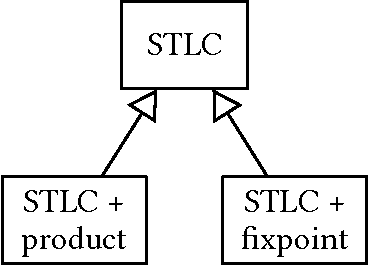
\includegraphics[scale=.48]{graphics/stlc-intro.pdf}
\end{wrapfigure}

%\noindent
%As an example, consider \cref{fig:STLC-example}, the simply typed
%lambda calculus (STLC) mechanized in Coq.
%A programming challenge there is to define distinct extensions of this
%STLC formalization to support distinct features,
%and then selectively compose these extensions to form new STLC variants.
As an example, the diagram to the right depicts an extensible
mechanization of the simply typed λ-calculus (STLC), using family
polymorphism.
An extension of STLC with products and another with iso-recursive types
can both inherit from the base STLC family:
they reuse mechanized metatheories,
from abstract syntax all the way to the type-safety theorem,
only adding new constructors to inductive types
and adding new cases to recursive functions and induction proofs
\emph{as needed} by an extension.

Integrating family polymorphism into a dependent type theory for
logical reasoning, however, poses significant technical challenges.
As we analyze, pillars of dependent type theories—including
inductive types, definitional equality, and logical consistency—are
all inimical to the kind of extensibility and family polymorphism
found in existing OO language designs.
Thus, our contributions include novel design recipes for dealing with
these challenges and strong meta\-theoretical guarantees on the
underlying logic.

\endgroup

Specifically, we make the following contributions.

\begin{itemize}[leftmargin=3.5ex]

\item We present the first language design that enables extensible
metatheory mechanization in a higher-order, dependent type theory with
inductive types (\cref{sec:lang-design}).
The language design reconciles the expressiveness enabled by
family polymorphism with the exactness of a proof assistant,
while retaining an idiomatic programming style.

\item We contribute a prototypical implementation of our language
mechanism as a Coq plugin (\cref{sec:coqimpl}). The plugin works by
compiling surface-language terms into Gallina terms parameterized by
extensibility hooks.

\item We capture the essence of the new language mechanism formally by extending
Martin–Löf type theory with family polymorphism and extensible inductive
types (\cref{sec:metatheory}).
We derive strong meta\-theoretical results including consistency and
canonicity.
We also formalize the translation implemented by the Coq plugin.

\item We present case studies of using our Coq plugin to mechanize
language metatheories (\cref{sec:coqexample}).
They show how our language design naturally solves the EP and
enables a high degree of reuse and extensibility
for proof engineering.

\end{itemize}

%\paragraph{Structure of the paper} We will quickly introduce Family
%Polymorphism and the challenges to adapt it into dependent type setting
%in \cref{sec:background+challenge}. After that, we will talk about the
%language design of family polymorphism in dependent type setting and the
%implementation of our Coq plugin in \cref{sec:coqimpl}. Then, we
%consider the meta-theory of incorporating family polymorphism into
%predicative MLTT, and deriving consistency and canonicity results in
%\cref{sec:metatheory}. \ref{sec:related-work} discusses related works
%and \ref{sec:conclusion} concludes.


